\documentclass{standalone}
\usepackage{tikz}

\begin{document}
\begin{tikzpicture}[scale=0.5]
    % Define the dimensions of the rectangle
    \def\rectWidth{5}
    \def\rectHeight{40}
    
    % Draw the rectangle
    \draw[fill=blue!20] (0,0) rectangle (\rectWidth,\rectHeight);
    
    % Calculate the position of each number
    \foreach \x [count=\xi from 1] in {5,7.6,9.8} {
        % Calculate the y-coordinate for the center of the number
        \pgfmathsetmacro{\yCoord}{(\rectHeight/2 - \rectHeight/20)*\xi}
        
        % Draw the number
        \node at (\rectWidth/2, \yCoord) {\x};
    }
    
    % Draw the arc
    \draw[thick,->] (0,0) arc (180:360:{\rectWidth/2} and {\rectHeight/2});
\end{tikzpicture}
\end{document}